%%=============================================================================
%% CAPITULO 3 -- PROCEDIMENTOS METODOLOGICOS
%% Esqueleto provisorio (dissertacao dummy): texto a ser desenvolvido.
%%=============================================================================

\section{Procedimentos metodológicos}

A pesquisa adota a Design Science Research (DSR) como método, organizando-se
na construção do artefato e em sua avaliação. A DSR não persegue a solução
ótima, mas a solução satisfatória, e exige que os parâmetros de aceitação sejam
fixados a priori: aqui, o artefato deve superar, na concordância com a
atribuição oficial do INEP, um método de recuperação lexical sem inteligência
artificial. Quanto à abordagem, a pesquisa é predominantemente quantitativa,
combinando técnicas computacionais de processamento com o confronto contra
referência documental externa ao sistema.

Os dados provêm de fontes secundárias e primárias: o acervo de videoaulas do
Preparatório ENEM do Canal Educação, acessível pelos metadados da plataforma de
hospedagem e pela transcrição automática do áudio, complementada pelos slides
de apoio; a matriz de referência do ENEM, em seus eixos cognitivos,
competências de área e 120 habilidades; e os microdados oficiais de itens de
prova do INEP, que registram a habilidade avaliada por cada questão em cada
edição do exame.

\subsection{Arquitetura do artefato}

A Figura~\ref{fig:pipeline} resume o fluxo de classificação. O artefato
organiza-se em quatro camadas funcionais: ingestão, representação semântica,
classificação e consulta. O modelo de codificação é o BGE-M3, modelo de
embeddings multilíngue de 1.024 dimensões empregado exclusivamente em
inferência, sem treinamento ou ajuste fino sobre os dados da pesquisa; a
cobertura multilíngue é necessária porque o acervo contempla disciplinas de
língua estrangeira, e a execução local dispensa a submissão de conteúdo público
a serviços externos.

\begin{figure}[htb]
  \caption{Fluxo de classificação das videoaulas do Canal Educação por habilidade do ENEM}
  \label{fig:pipeline}
  \centering
  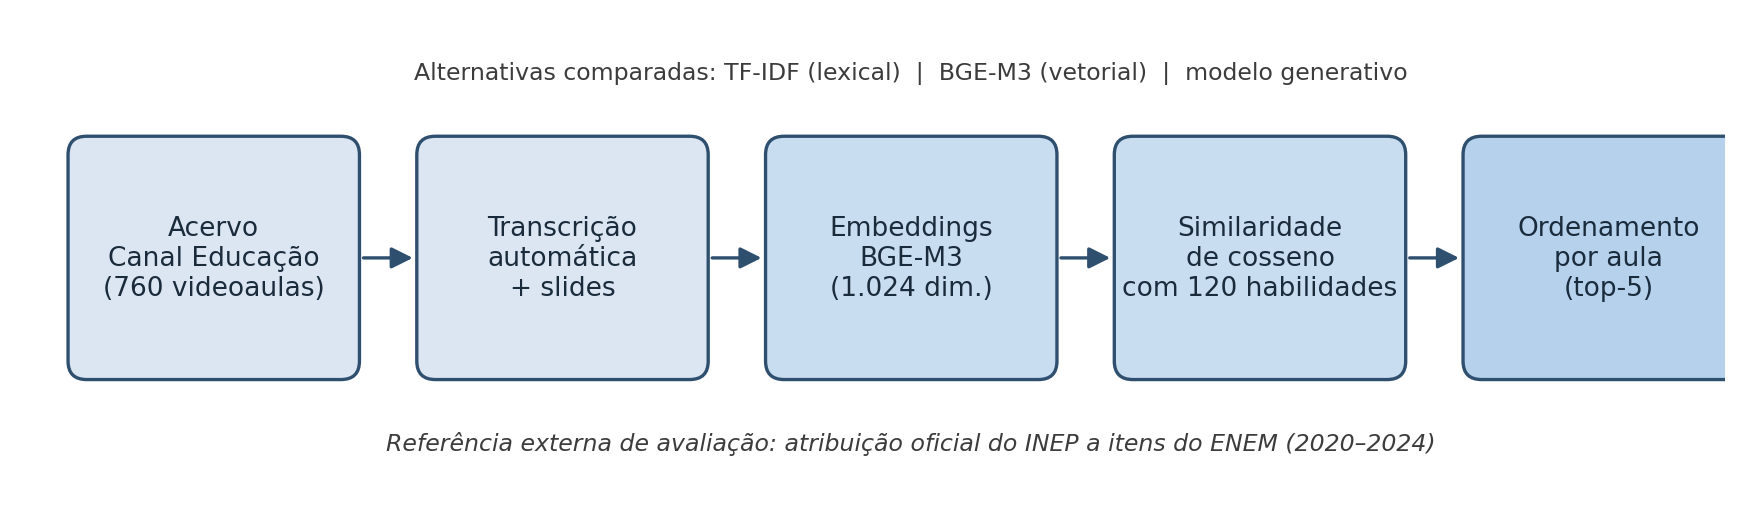
\includegraphics[width=\textwidth]{figuras/pipeline-classificacao.png}
  \fonte{Elaborado pelo autor (2026).}
\end{figure}

\subsection{Desenho da comparação}

A avaliação técnica confronta três alternativas sobre o mesmo conjunto de itens
e a mesma tarefa: a lexical, por TF-IDF, sem modelo de aprendizado, que
estabelece o piso atribuível à coincidência de vocabulário; a vetorial, com o
BGE-M3, que é o método em uso no artefato; e a generativa, por modelo
proprietário de grande porte fixado por identificador de versão datado. O
conjunto de descritores candidatos é idêntico em todas as condições e restrito
à área do item, com trinta habilidades por área. As condições lexical e
vetorial foram medidas nas cinco edições de 2020 a 2024, com 884 itens; a
generativa, na edição de 2023, com 178 itens.
